%!TEX root = ../Thesis.tex
\chapter{System Design}
The development of multi-agent systems requires spinning multiple instances of identical entities. In a real-world scenario, those entities would be real robots with their own computing unit connected to each other with some kind of networking. To simulate this scenario microservices approach will be used, as it allows to easily separate agents even on a single computer setup as well as put constrain on computing power and memory usage.
Cloud computing will also be used in this study and the micro-service approach is a native one for the cloud. Therefore all services around the agents will also be implemented as microservices.
\section{Microservices}
In recent years wide cloud adoption has caused huge momentum in adopting software architecture known as micro-services, as it is a native architecture for the cloud. This project will also adapt this architecture because part of the deployment is being done in the cloud, and a swarm of agents can also be simulated using this approach. Moreover, technologies such as kind and tilt made it easier to develop all services locally using the local Kubernetes cluster.

Micro-services are small autonomous services that cooperate with each other to create certain application logic\cite{building_microservices}. Usually, microservices are deployed as Linux containers and encapsulate logic for a single logical part of the solution. Those services are then communicating whit each other to build bigger, more complex systems.

\begin{figure}[H]
    \centering
    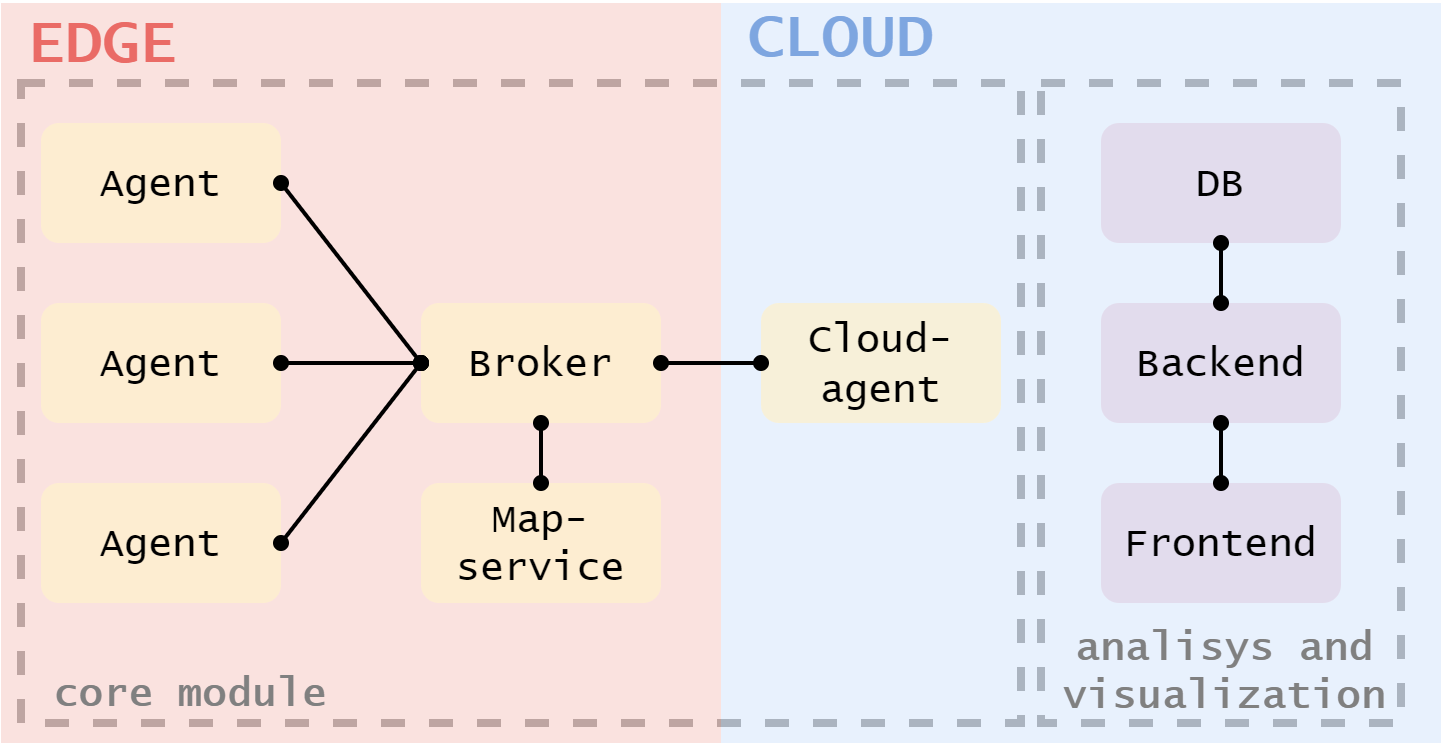
\includegraphics[width=\textwidth]{pictures/services.png}
    \caption{ Microservices system design }
    \label{fig:micro_services}
\end{figure}

\subsection{Agent}
The agent is a microservice which is implementing the logic of the entity which needs to plan a path.  It is meant to have limited resources to simulate a real-world scenario, and the number of its instances will vary.

When an agent is started, it doesn't belong to any swarm so it will start local discovery to find its peers. After peers are found, one of the agents has to be elected as a leader and therefore election algorithm will be initiated in one or multiple agents, so one of the agents will be elected to be a swarm leader. An agent will periodically poll his peers to check their liveness and this behavior will be referred to as a liveness check.

This entity contains also all algorithms meant for path planning as in a base case scenario, computation will take place in the agent to obtain the path.

\subsection{Cloud-agent}
The cloud-agent is a service that provides computational resources to offload the workload from agents. It is designed to have significantly more computing power than the agents, but it may be located in a different geographical location, which could result in latency issues when transmitting data back and forth.

In order to communicate with the agents, the cloud-agent uses the cloud-broker as a medium. The cloud-broker acts as an intermediary, enabling the cloud-agent and the agents to exchange messages and data.

The cloud-agent is deployed in the cloud and is intended to be used for performing computationally intensive tasks that would be too resource-intensive for the agents to handle on their own. By offloading these tasks to the cloud-agent, the agents are able to operate more efficiently and effectively.

\subsection{Broker}
This service plays a crucial role in the system, it is responsible for facilitating communication between various services. It is deployed both in the cloud and in local environments, and the two entities are connected by a bridge. The bridge serves as a single connection point between the cloud and the edge, allowing the two to communicate and exchange data.

Alternatively, the cloud and local services can also cross-subscribe to both brokers, allowing them to communicate directly with each other. The service uses a publish-subscribe (pub/sub) approach to handle and distribute messages between the different services.

The service acts as an intermediary, enabling services to exchange messages and data without the need for direct communication. This can help to reduce the complexity of the overall system and make it more scalable and resilient.

\subsection{Map-service}
This service is responsible for generating maps and spawning agents within them. When an agent is first created, it does not have any map assigned to it. The leader agent will trigger the generation of a new map by sending a message to the map-service. The map-service is responsible for creating the map and spawning the agent within it. Communication between the map-service and the agents is facilitated by the broker service. The broker service acts as an intermediary, enabling the map-service and the agents to exchange messages and data. It is through the broker service that the map-service sends the necessary information to the agents and receives requests and updates from them.

The map-service serves as a substitute for sensing for the agent, as it provides the robot with all the necessary information for determining its position on a global map. In addition to generating new maps, the map-service also stores pre-defined maps that can be adopted by the agent upon request.

It is possible for the map-service to spawn agents in places that are not reachable from the goal. This is a valid scenario as not all points on the map might be reachable. The map-service is a crucial component for enabling agents to navigate and interact with their environment.

\subsection{Backend}
This service is designed to gather data and facilitate communication with a core module service (such as an agent or map service) through a cloud broker. The service exposes endpoints through a REST API(appendix \ref{app:app_01}), which can be accessed by a frontend application. It also forwards requests to an MQTT broker.

In addition to interacting with other services, this service also receives data from various entities and stores it in a database. The backend of this service is deployed in the cloud, and the endpoints are accessible to end-users. It is equipped with a database for storing data. The database is attached to the service, which means that it is directly accessible and can be used for storing and retrieving data as needed. The service is designed to receive data from various entities, and it stores this data in the attached database for later use.

This service acts as an intermediary between the frontend, the core module service, and the MQTT broker, allowing them to communicate and exchange data. It is deployed in the cloud and connected to a cloud broker, which enables it to access resources and services hosted in the cloud.

\subsection{Frontend}
The frontend of this service is a graphical interface that is deployed as a web service. It is accessed by end users through a web browser and is used to trigger specific actions and perform raw data visualization.

The frontend is responsible for taking input from the end user and sending requests to the backend service through its API. It is also used for visualizing raw data, allowing the end user to view and analyze the data in various ways.

The frontend is deployed in the cloud and is exposed to end users over the internet. Its capabilities are further explained in the \hyperref[sec:0308]{visualization section} section of the documentation.

Frontend serves as the interface between the end user and the backend service, allowing the end user to interact with the service and access its functionality. It is an important component of the service, as it enables the end user to perform various actions and view raw data in an intuitive and user-friendly way.


\section{Cloud Computing}
The objective of the design of cloud deployments is to achieve cloud agnosticism, which implies that it can operate seamlessly with any cloud provider with minimal or no modifications. To achieve this, all services are intended to be deployed within a Kubernetes cluster, regardless of the location or configuration of the cluster. This is feasible as most major cloud providers offer Kubernetes as a Service (KaaS), and it is also widely available among smaller providers.

The comprehensive design of the cloud services is depicted in Figure \ref{fig:cloud_services}. The communication between the various services is established in two ways:
\begin{itemize}
    \item Through the Cloud Broker: The backend and cloud-Agent services are both subscribers to a set of topics and exchange information through MQTT messages sent to the Cloud Broker.
    \item Through REST Endpoints: The backend services expose REST endpoints which are consumed by the frontend. The frontend is designed to solely serve HTML documents and function as a consumer of the backend endpoints.
\end{itemize}

\begin{figure}[H]
    \centering
    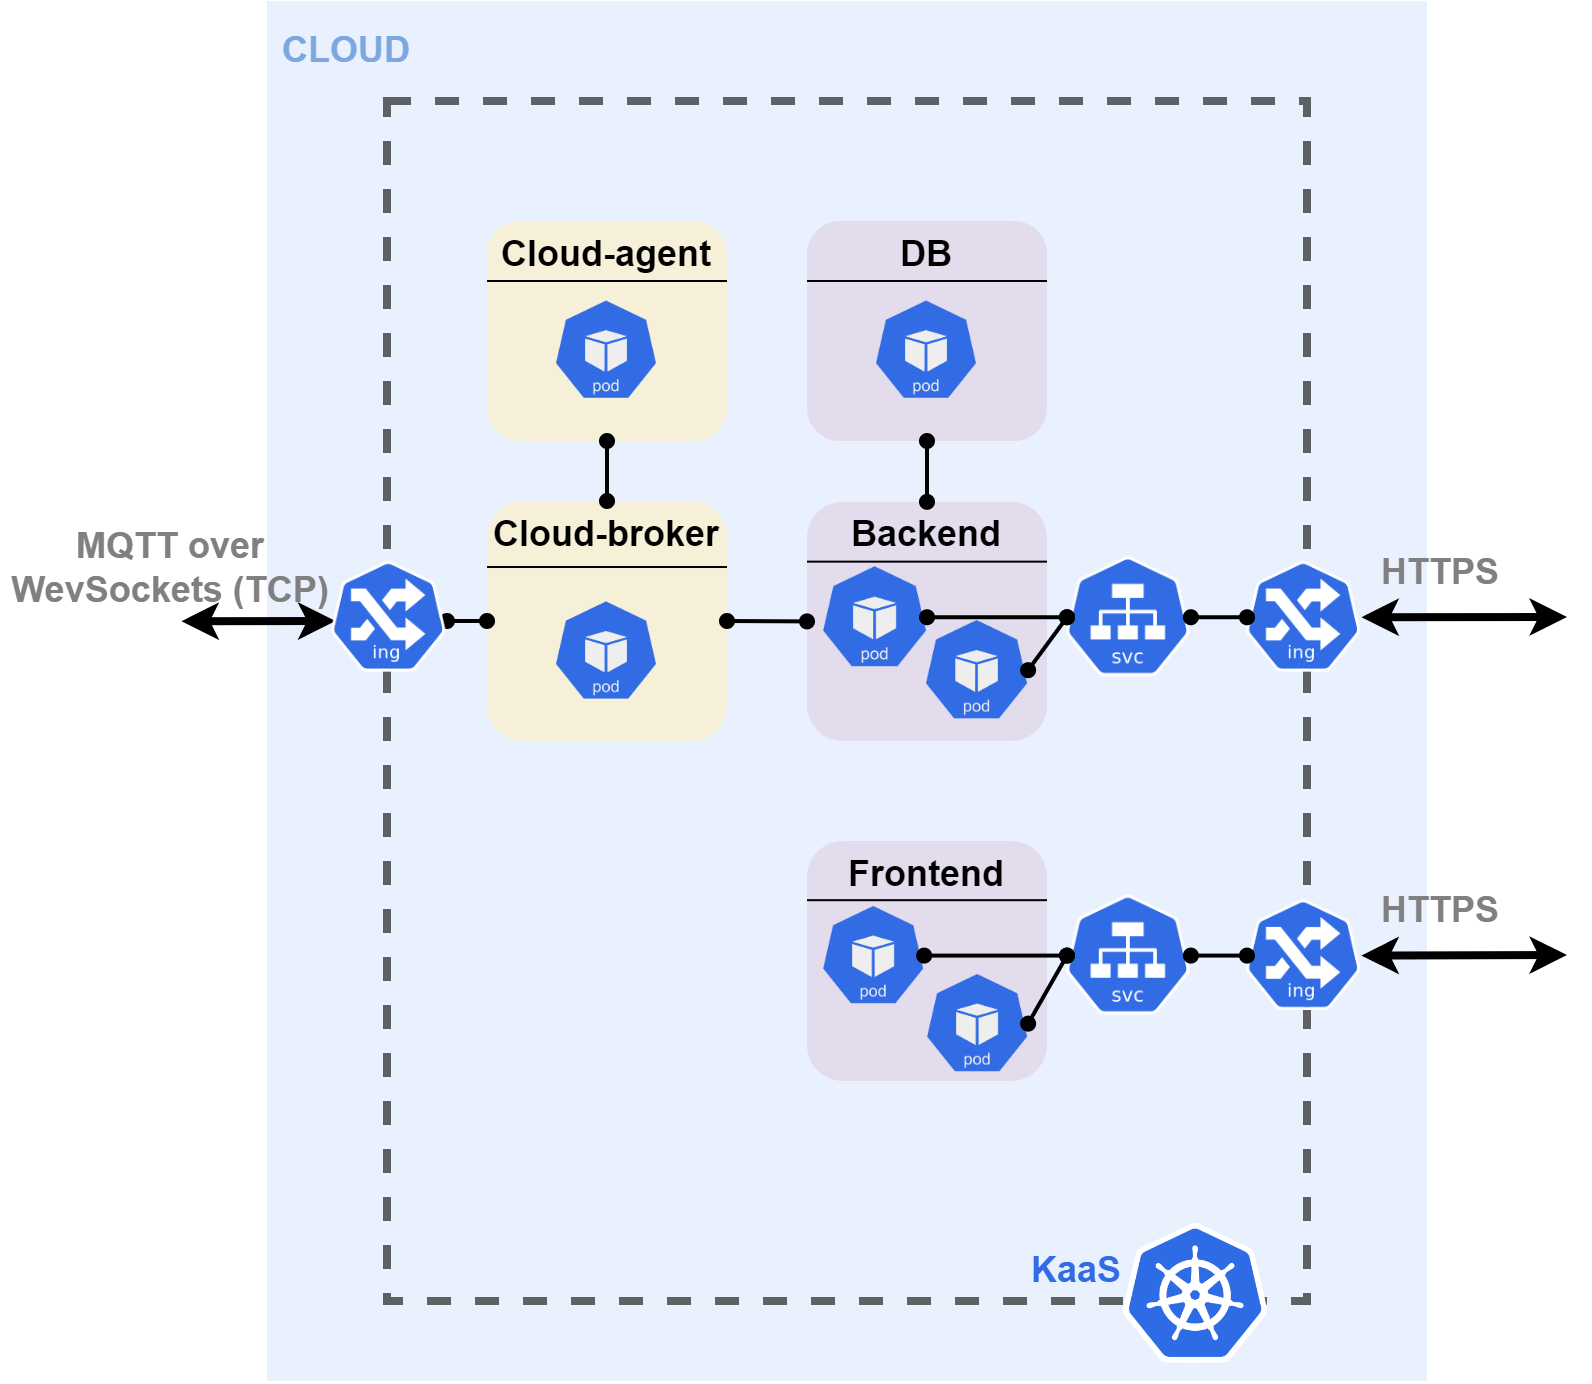
\includegraphics[width=0.85\textwidth]{pictures/cloud_services.png}
    \caption{Cloud services system design}
    \label{fig:cloud_services}
\end{figure}

In this system design, three endpoints are exposed to external traffic, which originates from outside of the cluster. These include two HTTP/HTTPS(Hypertext Transfer Protocol) endpoints for the Backend and Frontend and one WebSocket endpoint for MQTT messages that are sent to the cloud broker. HTTP/HTTPS traffic for frontend and backend is served through the use of ingress resources within the cluster. The traffic is forwarded via a reverse proxy (NGINX) to a Kubernetes service, which then distributes the request among the pods. The default ingress resource is designed to handle only HTTP/HTTPS requests and does not allow for any other protocol.

For the MQTT protocol, which is transported over TCP protocol, a NodePort \cite{kubernetes_docs} would typically be used to expose the service to the outside world. This maps pod ports to ports of the node in the cluster. However, some cloud providers do not permit the use of NodePorts, so a more flexible option was chosen, which involves bootstrapping the MQTT protocol over WebSockets and using ingress resources to handle external traffic coming to the cluster. This approach allows for the handling of MQTT traffic in a way that is compatible with the ingress resource and does not require the use of NodePorts.

\section{Edge Computing}
Agents, a local broker, and a map service are deployed on-premises and can facilitate the computation of the path in this setup. Agents can communicate with each other to agree on who will initiate the computation. Figure \ref{fig:local_services} shows how local services are deployed. Local broker and map services need to be accessible for all agents to communicate and map selection and therefore in most cases those services would be deployed on a stand-alone server in the same subnet as agents.

\begin{figure}[H]
    \centering
    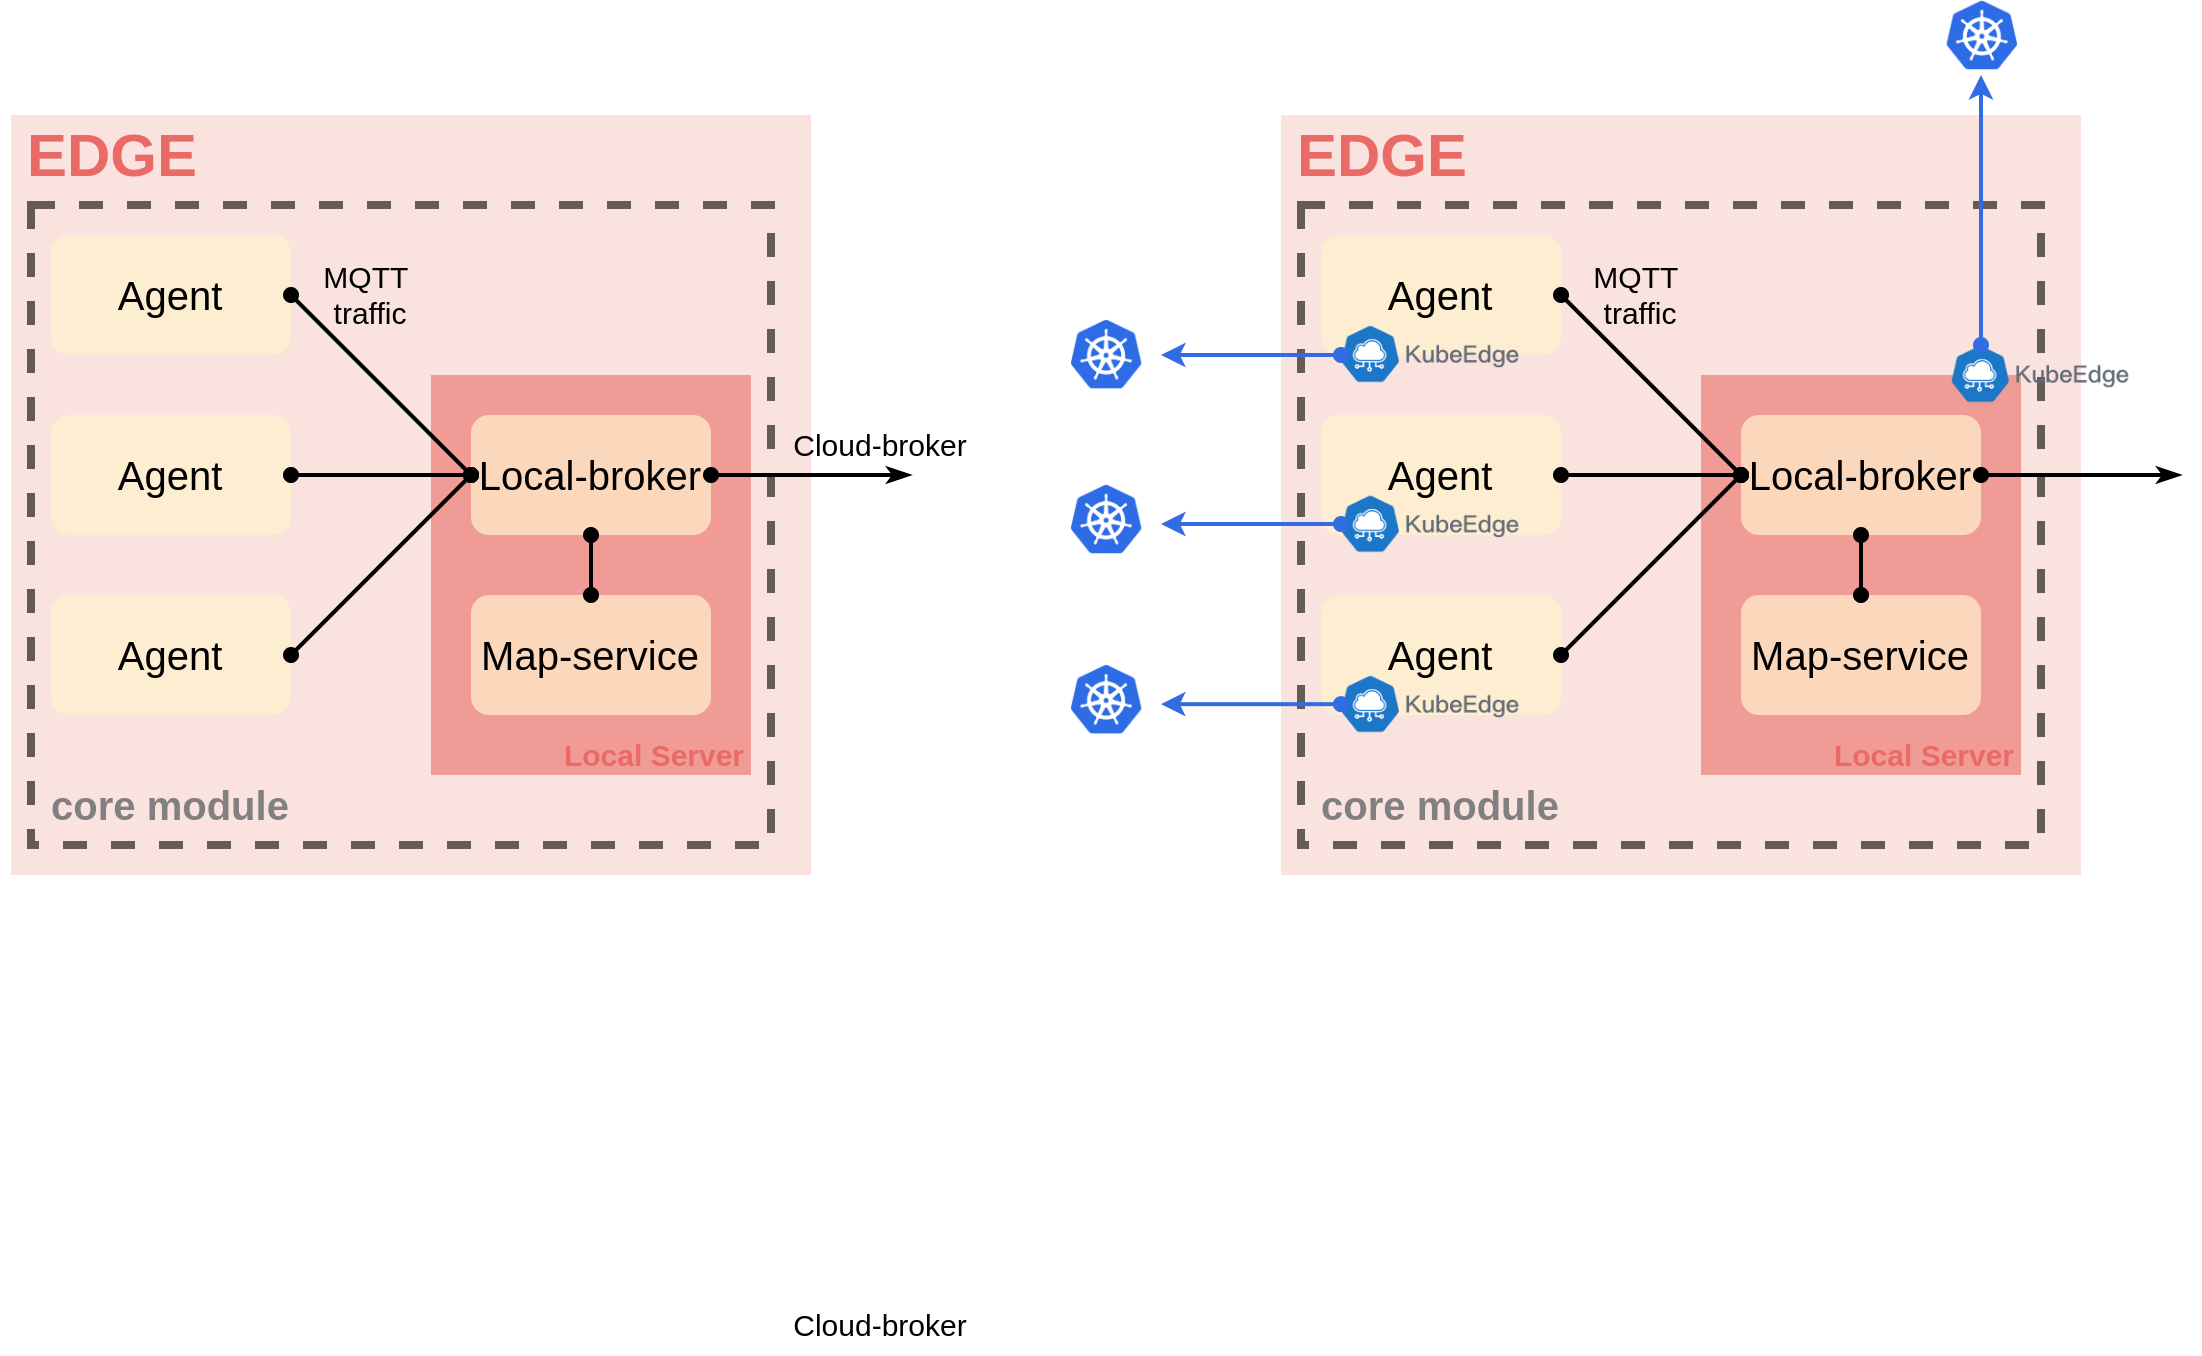
\includegraphics[width=0.5\textwidth]{pictures/local_service.png}
    \caption{Local services system design}
    \label{fig:local_services}
\end{figure}

This design can be extended, by deploying an edge agent on the same server as a map service and a broker. It would allow performing path computation with help of an edge agent which would have a higher resource profile than agents.

Agents can be deployed in a different way, depending on implementation. Preferably it should be a single binary package that could be deployed on machines with low resource profiles. All the agents need to have an ID or NAME assigned to them, and those have to be unique in the scope of the system. They should also be given information about the IP address or URL of the local broker and a way to authenticate themselves. 

Map service and broker are more flexible in case of deployment because those services would probably be deployed on a stand-alone server with a high resource profile. Recommended way would be to use a containers orchestrator such as solutions like Kubernetes or docker swarm and deploy the as containers/pods. It would assure the reliability and maintainability of those services. Otherwise, those can also be deployed on bare metal or in virtual machines.

\section{Communication Between Agents}
The broker is a critical component in the proposed system design, responsible for facilitating communication between microservices. In an on-premises system, the broker is deployed to allow communication between agents and map service. In an industry setup, it would typically be deployed on a stand-alone server located in the same subnet as the agents. It acts as a middleman, receiving all messages and redirecting them to the appropriate parties involved in the communication process. One broker can be used to support multiple systems, as long as they are connected to the same subnet as the broker. This is made possible by the messaging scheme, which is distinctive for every system (as described in section \ref{sec:app_02}), allowing the broker to correctly route the request. The broker is an essential component of the system, ensuring that all mobile robots can communicate effectively and enabling the system to function as intended.

The MQTT protocol was selected for communication between the agents because it is extremely lightweight and suitable for IoT communication. This makes it an ideal choice for supporting agents with very limited resources, such as those with limited memory, CPU, or bandwidth. This protocol is designed to be efficient in terms of both bandwidth and power usage, which makes it well-suited for use in a large-scale, distributed system like the one proposed here.

\section{Leader Election}
\begin{figure}[H]
    \centering
    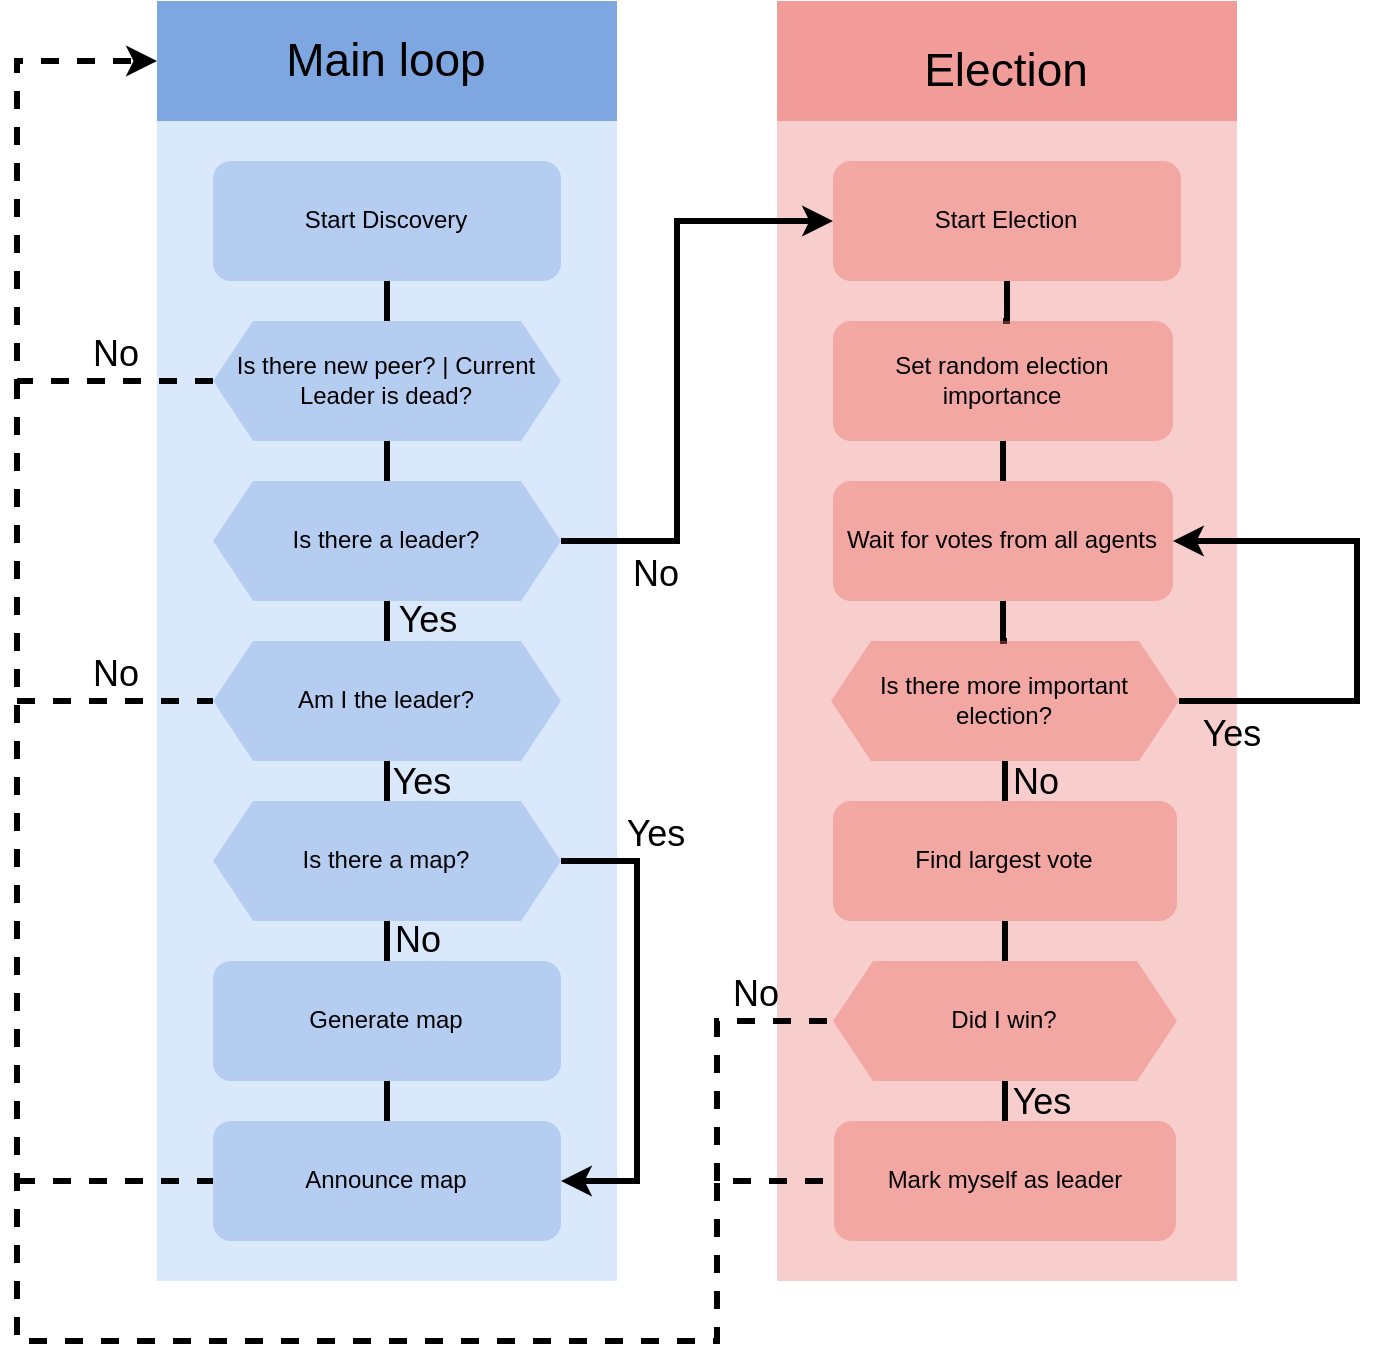
\includegraphics[width=0.8\textwidth]{pictures/election_logic.png}
    \caption{ Election logic}
    \label{fig:election_logic}
\end{figure}


\section{Map Design}
This section focuses on the design of the map representation used in the multi-agent system. The map serves as a representation of the possible location of the agents in a discrete space. The initial map generated for the agents will indicate the starting and finishing points for each agent. Additionally, different algorithms may require the map to be translated into different forms, such as a graph. These different forms of representation are necessary to enable the efficient operation of specific algorithms. 

\subsection{Gridmap}
A grid map is a representation of the possible location of the agent in a discrete space. On the initial map generated for the agents, starting and finishing points of each agent will be indicated. A map will also include an indication of unreachable spots, which will be referred to as "walls" or "obstacles". Two possible map standards will be implemented: space-separated map and JSON-based map. The space-separated map is meant for creating and storing persistent maps, as it is also human-readable. The JSON-based map is mostly meant for machine-to-machine communication, as it is easily parsable. Conversion between those maps, as well as storage, will happen in the map service. It will be also served to the agents from this microservice, which will have the possibility of generating random maps and spawning agents on it.

Before executing an algorithm, the map will have to be translated to a graph, where each tile of the grid map represents one node of the graph. Edges of the graph represent possible agent movement. Two possible modes will be available: with and without diagonal movement \ref{fig:map_2D}. By default, algorithms will use mode without diagonal moves.

\begin{figure}[H]
    \centering
    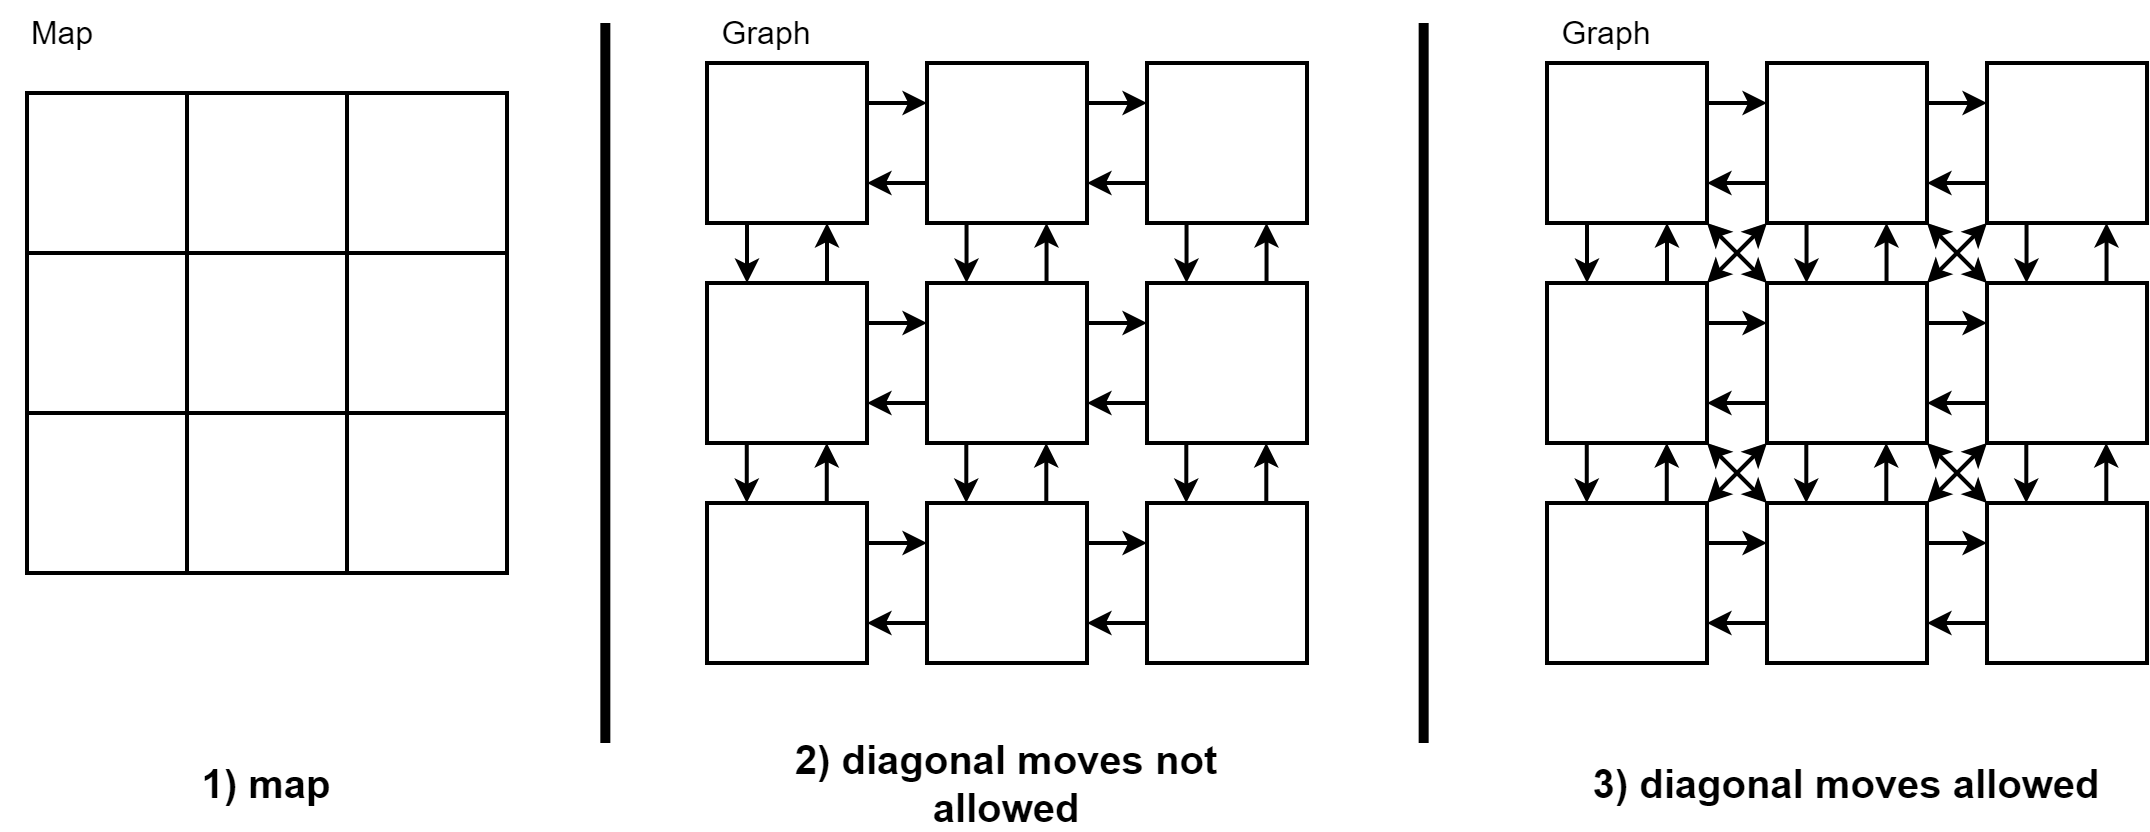
\includegraphics[width=\textwidth]{pictures/map_2d.png}
    \caption{ 2D map to graph translation }
    \label{fig:map_2D}
\end{figure}

Each tile represents the node and it is connected with two edges to neighboring tiles, which represents the possibility of two-way movement from and to neighboring tiles. 


\subsection{Gridmap for CA* algorithm}
For CA* algorithm map has to be translated into a 3d grid map where every layer is a representation of the possible location of the agent in a particular time frame and therefore time becomes the third dimension in a graph. Similar to in a 2d grid map there are two possible modes which are represented in the figure below. An agent can only move in one direction vertically as each level corresponds to one moment in time. Other tiles on each level are connected in the same way as in figure \ref{fig:map_2D}.
\begin{figure}[H]
    \centering
    \includegraphics[width=\textwidth]{pictures/map_3D.png}
    \caption{ 3D map to graph translation }
    \label{fig:map_3D}
\end{figure}
After the path is planned for specific agents, it has to be marked as an obstacle so agents which are planning their paths, later on, would be aware of unreachable/occupied tiles.

\subsection{CA* front collision problem}
Planning multiple agents' paths on a single map leads to a problem when agents are colliding with each other because they are moving in the opposite direction on the same column or row. This situation is shown in figure \ref{fig:head_collision}. Both agents assume that the tile in front of them is not occupied, which is a valid assumption. However, as this is a discrete model, a collision occurs between timeframes. To mitigate this problem, after the path is planned edges in the opposite direction of agent movement need to be removed.
\begin{figure}[H]
    \centering
    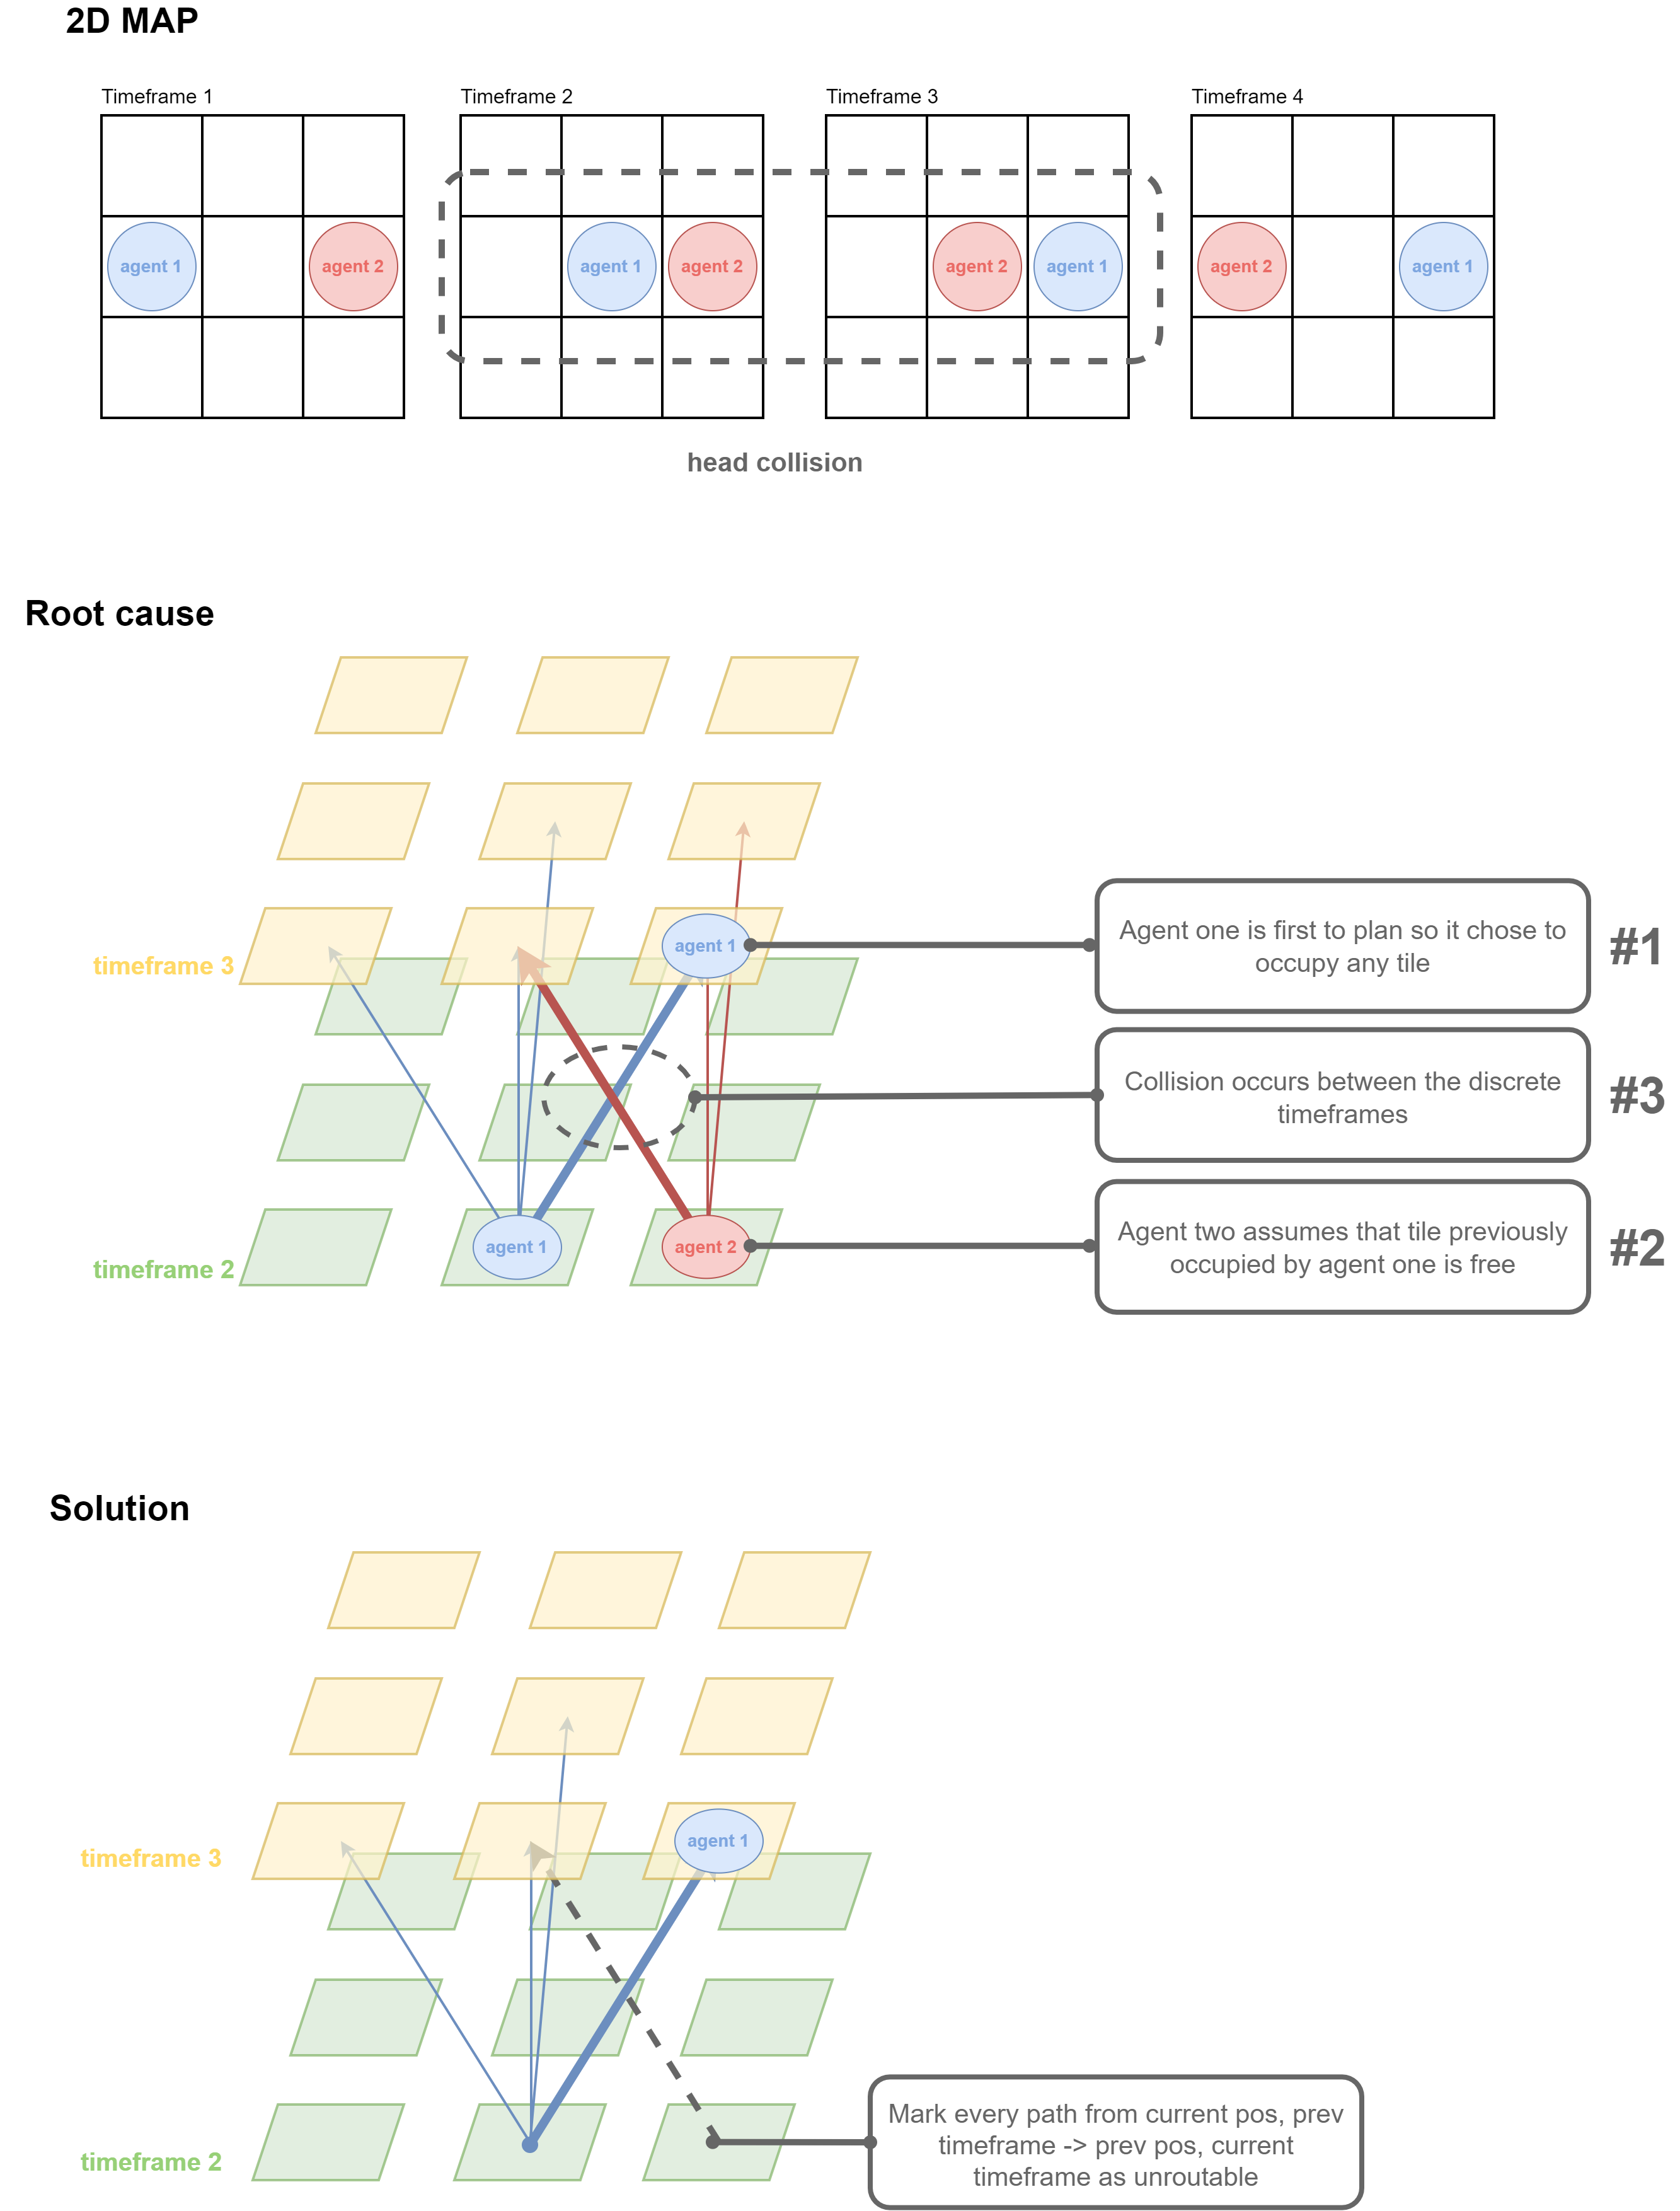
\includegraphics[width=0.7\textwidth]{pictures/head_collision_problem.png}
    \caption{ CA* head collision problem}
    \label{fig:head_collision}
\end{figure}

\section{Liveliness Algorithm}
Map 2d is a representation of possible location of the agent.
\begin{figure}[H]
    \centering
    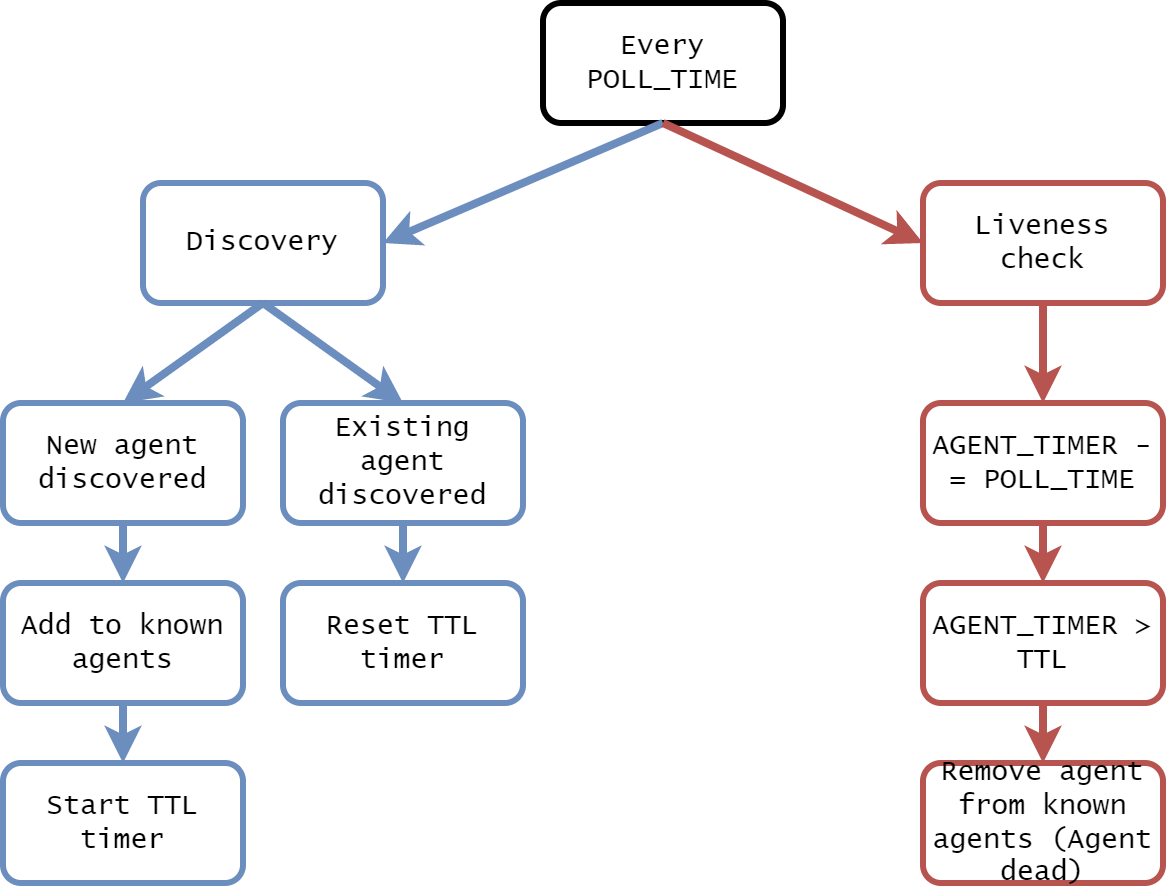
\includegraphics[width=0.8\textwidth]{pictures/agent_ttl.png}
    \caption{ Liveness check }
    \label{fig:liveness_check}
\end{figure}


\section{Visualization}
Maps and paths will be visualized in form of web application. It should be accessible from internet and connect to specific system to fetch live data. Mock of the visualization is shown on the figure \ref{fig:vis_mock}. 

\begin{figure}[H]
    \centering
    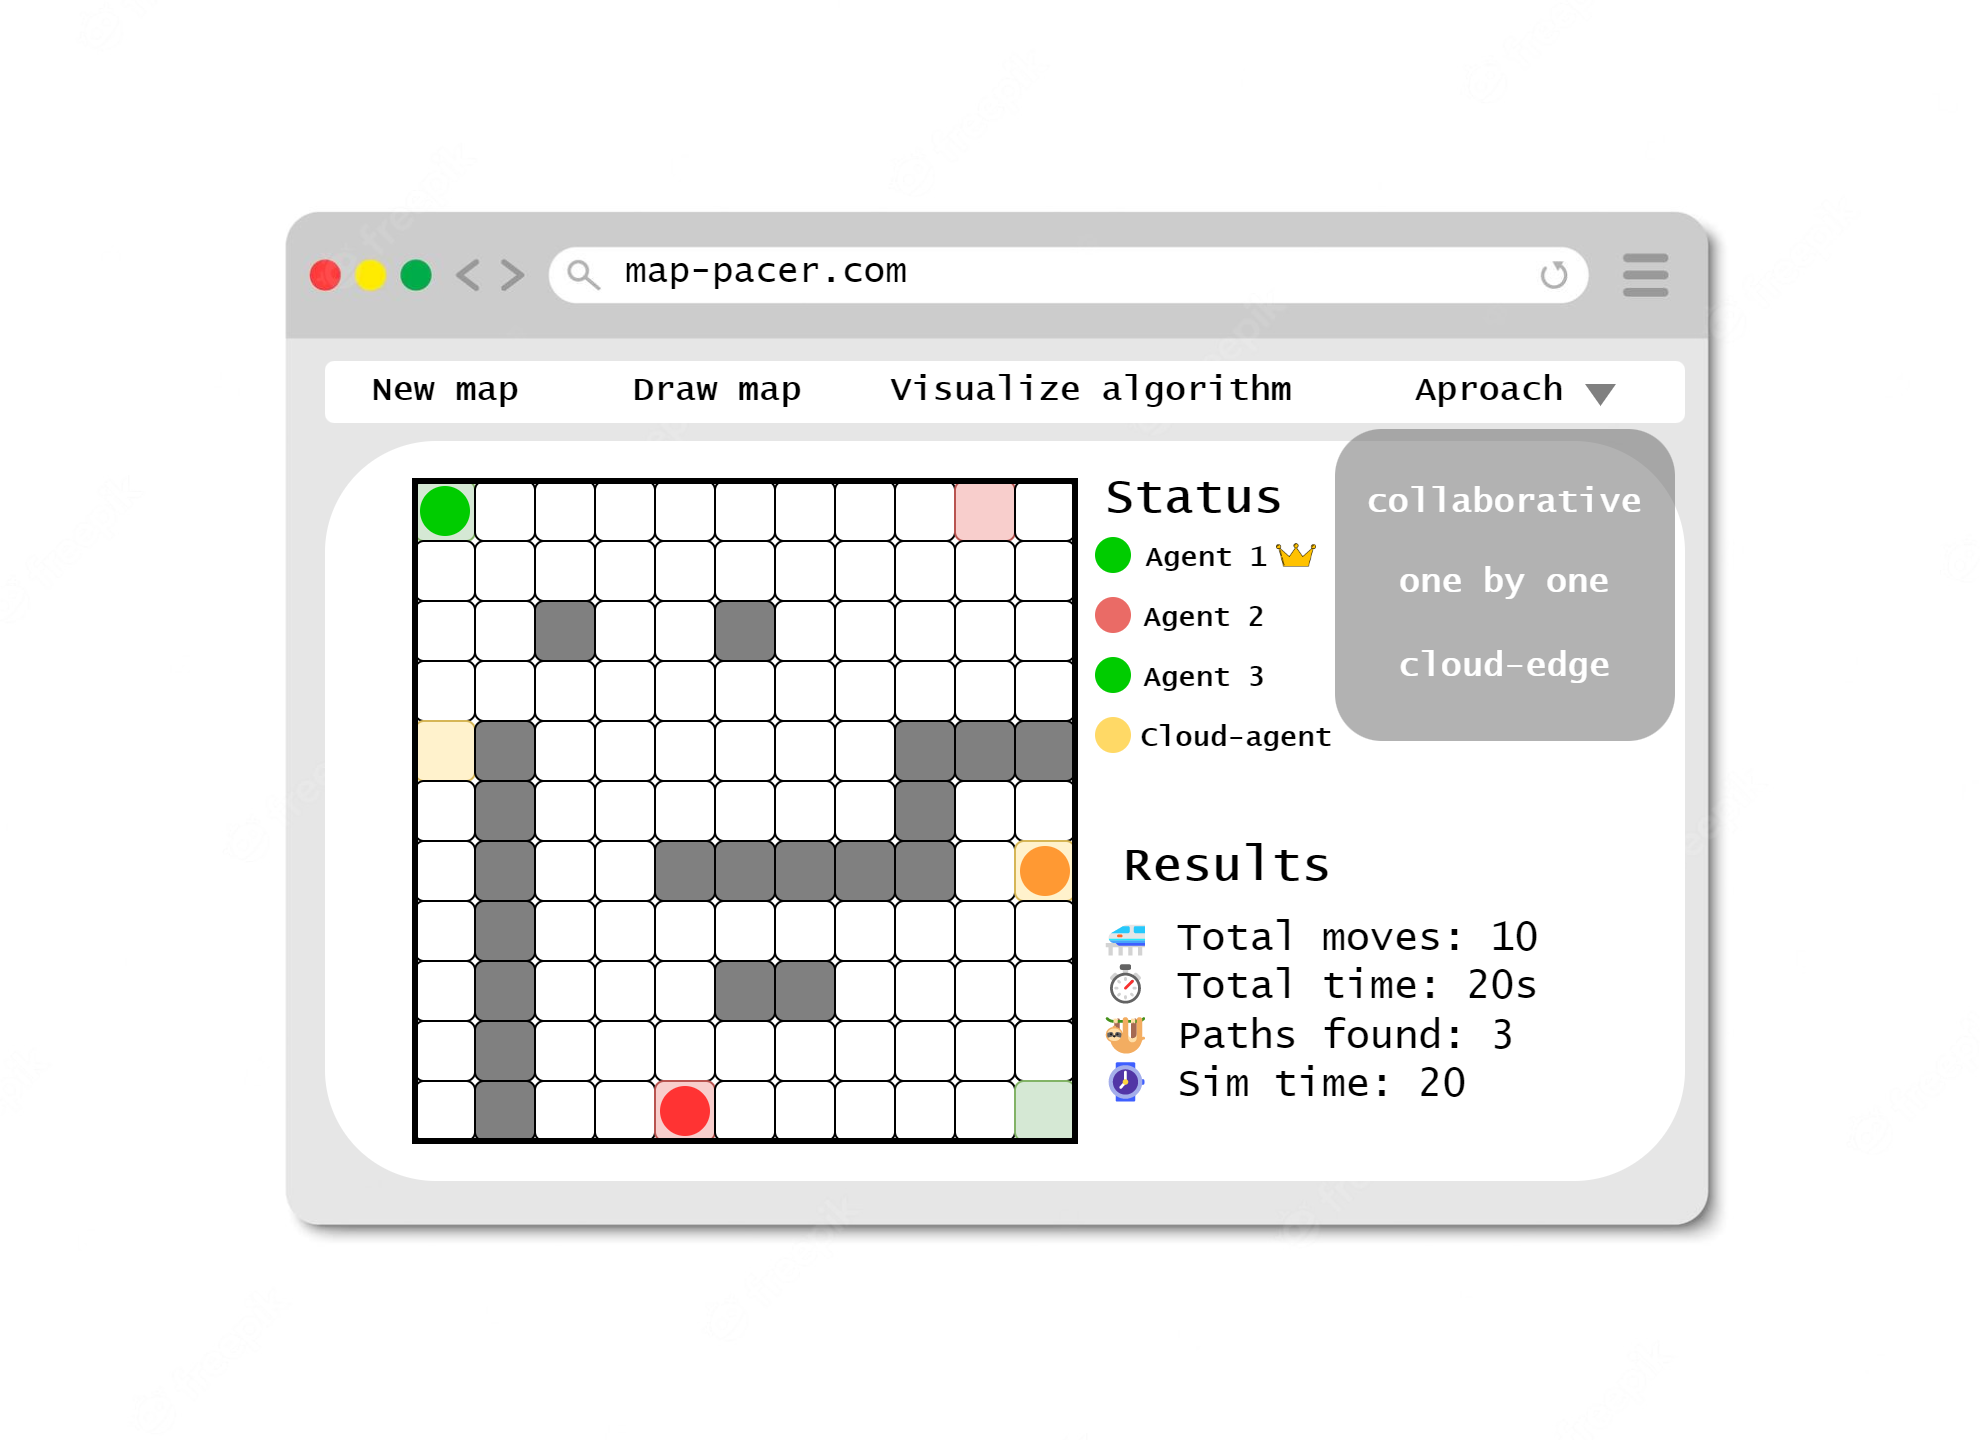
\includegraphics[width=\textwidth]{pictures/frontenf_mock.png}
    \caption{ Mock of the visualization }
    \label{fig:vis_mock}
\end{figure}

Graphical interface will be centered around gridmap which indicates positions and goal of all the agent(marked as coloured dots). On a side of the map will be status of the agent, indication of current leader and some details about result of the algorithm.

Through webapp, user will be able to(core functionality):
\begin{itemize}
\itemsep0em 
    \item Generate new map(random or predefined map)
    \item Create new map
    \item Select algorithm
    \item Visualize algorithm
\end{itemize}
Additional features:
\begin{itemize}
\itemsep0em 
    \item Access map creator, to specify own map.
    \item Choose among different systems(multi tenancy).
    \item Reply visualization.
\end{itemize}